%
% nullstellenschachtelung.tex
%
% (c) 2020 Prof Dr Andreas Müller, Hochschule Rapperswil
%
\begin{frame}
\frametitle{Nullstellen von $f(x)$ und $f'(x)$}
\begin{block}{Nullstellen sind geschachtelt}
Zwischen zwei Nullstellen von $f(x)$ gibt es immer eine Nullstelle 
von $f'(x)$.
\end{block}
\begin{center}
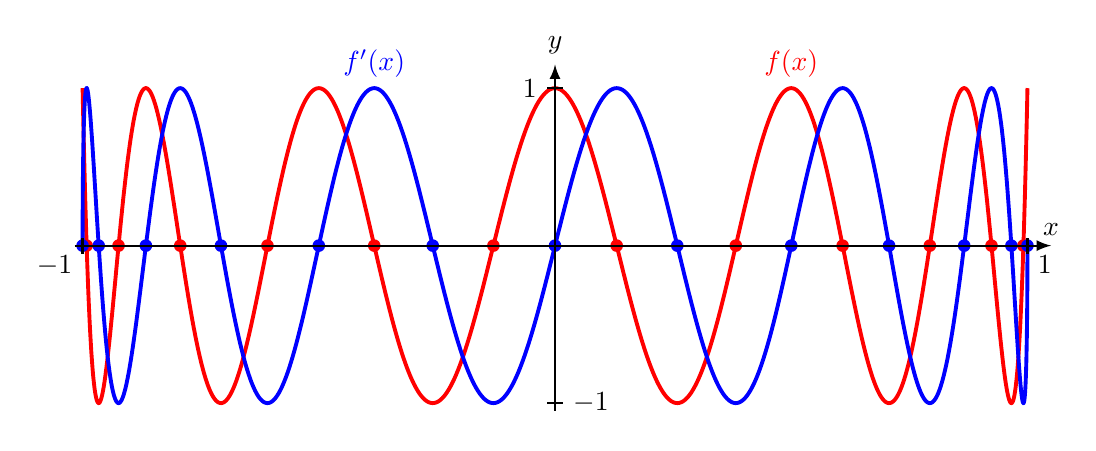
\begin{tikzpicture}[>=latex,thick]
\def\N{12}

\uncover<2->{
\node[color=red] at ({6*cos(180*(4/\N)},2) [above] {$f(x)$};
\draw[color=red,line width=1.4pt]
	plot[domain=0:180,samples=1000]
		({6*cos(\x)},{2*cos(\N*\x)});
\foreach \k in {1,...,\N}{
	\fill[color=red] ({6*cos(180*(2*\k-1)/(2*\N))},0) circle[radius=0.08];
}
}

\uncover<3->{
\node[color=blue] at ({6*cos(180*((2*8-1)/(2*\N))},2) [above] {$f'(x)$};
\draw[color=blue,line width=1.4pt]
	plot[domain=0:180,samples=1000]
		({6*cos(\x)},{-2*sin(\N*\x)});
\foreach \k in {0,...,\N}{
	\fill[color=blue] ({6*cos(180*(\k/\N))},0) circle[radius=0.08];
}
}

\draw[->] (-6.1,0)--(6.3,0) coordinate[label={$x$}];
\draw[->] (0,-2.1)--(0,2.3) coordinate[label={$y$}];
\draw (-6,-0.1)--(-6,0.1);
\node at (-6,0) [below left] {$-1$};
\draw (6,-0.1)--(6,0.1);
\node at (6,0) [below right] {$1$};

\draw (-0.1,-2)--(0.1,-2);
\node at (0.1,-2) [right] {$-1$};
\draw (-0.1,2)--(0.1,2);
\node at (-0.1,2) [left] {$1$};

\end{tikzpicture}
\end{center}
\end{frame}
